\section{空间向量的应用}

本节要点:
\begin{itemize}
    \item 掌握空间点线面的方程;
    \item 熟练掌握使用向量判断空间点线面的关系。
\end{itemize}

%============================================================
\subsection{用空间向量研究直线、平面的位置关系}

首先定义点、线、面的向量表达式。

{\bf 空间中的点}

直接用向量或其坐标表示:
\[
\overrightarrow{OP} \qquad \boldsymbol{p} \qquad \left( x_{\boldsymbol{p}},y_{\boldsymbol{p}},z_{\boldsymbol{p}} \right)
\]

{\bf 空间中的直线}

直线的定义是和给定点$P_0$构成的向量与给定向量$\boldsymbol{n}$平行的所有点的集合,即:
\[
\overrightarrow{P_0P}=\lambda \boldsymbol{n} \quad \text{或} \quad \left( x-x_0,y-y_0,z-z_0 \right) =\lambda \left( A,B,C \right)
\]
展开后得空间直线方程:
\[
\frac{x-x_0}{A}=\frac{y-y_0}{B}=\frac{z-z_0}{C}
\]
其中:
\begin{itemize}
    \item $\boldsymbol{n}=\left( A,B,C \right) $:直线的方向;
    \item $\left( x_0,y_0,z_0 \right) $:直线上一点$P_0$的坐标。
\end{itemize}

{\bf 空间中的平面}

平面的定义是和给定点$P_0$构成的向量与给定向量$\boldsymbol{n}$垂直得所有点得集合,即:
\[
\overrightarrow{P_0P}\cdot \boldsymbol{n}=0 \quad \text{或} \quad A\left( x-x_0 \right) +B\left( y-y_0 \right) +C\left( z-z_0 \right) =0
\]
展开后得到空间平面的一般方程:
\[
Ax+By+Cz+D=0
\]
其中:
\begin{itemize}
    \item $\boldsymbol{n}=\left( A,B,C \right) $:平面的法线方向;
    \item $\left( x_0,y_0,z_0 \right) $:平面上一点$P_0$的坐标。
\end{itemize}
特别地,当平面和{\it xyz}轴分别交于$x_0,y_0,z_0$时,则可以写成截距式:
\[
\frac{x}{x_0}+\frac{y}{y_0}+\frac{z}{z_0}=0
\]

\begin{tcolorbox}
以上定义中,关键在于点和方向。点好理解,直线或平面上的点,直线的方向也好理解,面的方向是第一次碰到,我们取平面的法线的方向作为平面的方向。还要注意,高中阶段的方向,不分正反!
\end{tcolorbox}

\begin{theorem}
根据以上定义,我们不难得到直线和平面关系的判定定理:
\begin{itemize}
    \item 若$\boldsymbol{l}_1=\lambda \boldsymbol{l}_2$,则两直线$l_1,l_2$平行;
    \item 若$\boldsymbol{l}\cdot \boldsymbol{n}=0$,则直线$l$平面$\alpha $平行;
    \item 若$\boldsymbol{n}_{\alpha}=\lambda \boldsymbol{n}_{\beta}$,则两平面$\alpha ,\beta $平行;
    \item 若$\boldsymbol{l}_1\cdot \boldsymbol{l}_2=0$,则两直线$l_1,l_2$垂直;
    \item 若$\boldsymbol{l}=\lambda \boldsymbol{n}$,则直线$l$平面$\alpha $垂直;
    \item 若$\boldsymbol{n}_{\alpha}\cdot \boldsymbol{n}_{\beta}=0$,则两平面$\alpha ,\beta $垂直。
\end{itemize}
\end{theorem}

\begin{table}[h]
\centering
\begin{tabular}{ccc}
    \toprule
     & 平行 & 垂直\\
    \midrule
    线线$l_1,l_2$ & $\boldsymbol{l}_1=\lambda \boldsymbol{l}_2$ & $\boldsymbol{l}_1\cdot \boldsymbol{l}_2=0$\\
    线面$l,\alpha $ & $\boldsymbol{l}\cdot \boldsymbol{n}=0$ & $\boldsymbol{l}=\lambda \boldsymbol{n}$\\
    面面$\alpha ,\beta $ & $\boldsymbol{n}_{\alpha}=\lambda \boldsymbol{n}_{\beta}$ & $\boldsymbol{n}_{\alpha}\cdot \boldsymbol{n}_{\beta}=0$\\
    \bottomrule
\end{tabular}
\end{table}

%============================================================
\subsection{用空间向量研究距离、夹角问题}

如下图,点$P$到直线和平面的距离表达式:

\begin{figure}[h]
\centering
\begin{minipage}{.49\textwidth}
\centering
\begin{tikzpicture}[line join=round, scale=0.5]
\coordinate[label=below:{$A$}]                (A)  at (0,0);
\coordinate[label=below:{$Q$}]                (Q)  at (4,0);
\coordinate[label=right:{$P$}]                (P)  at (4,3);
\coordinate[label=right:{$\boldsymbol{l}_0$}] (l0) at (6,0);
\draw[thick] ($(A)!-0.5!(Q)$)--($(A)!1.5!(Q)$);
\draw[thick,-stealth] (A)--(P);
\draw[dashed] (Q)--(P);
\end{tikzpicture}
\end{minipage}
\begin{minipage}{.49\textwidth}
\centering
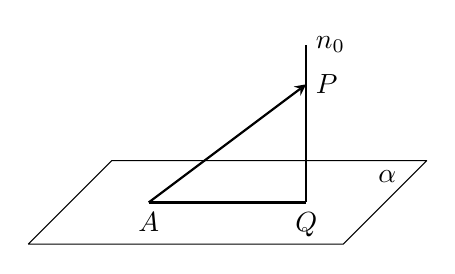
\begin{tikzpicture}[style={x={(-135:0.5)},y={(1cm,0)},z={(0,1cm)}}, line join=round, scale=0.5]
\draw (3,-2,0)--(3,6,0)--(-3,6,0)--(-3,-2,0)--(3,-2,0);
\coordinate[label=below:{$\alpha $}]          (a)  at (-3,5,0);
\coordinate[label=below:{$A$}]                (A)  at (0,0,0);
\coordinate[label=below:{$Q$}]                (Q)  at (0,4,0);
\coordinate[label=right:{$P$}]                (P)  at (0,4,3);
\coordinate[label=right:{$\boldsymbol{n}_0$}] (n0) at (0,4,4);
\draw[thick] (A)--(Q);
\draw[thick,-stealth] (A)--(P);
\draw[thick] (Q)--(n0);
\end{tikzpicture}
\end{minipage}
\end{figure}

\[
PQ=\sqrt{\overrightarrow{AP}^2-\left( \overrightarrow{AP}\cdot \boldsymbol{l}_0 \right) ^2} \qquad \qquad PQ=\left| \overrightarrow{AP}\cdot \boldsymbol{n}_0 \right|
\]
其中:
\begin{itemize}
    \item $\boldsymbol{l}_0$:直线的单位方向向量;
    \item $\boldsymbol{n}_0$:平面的单位法向方向向量。
\end{itemize}

~

如下图,线线、线面、面面夹角的余弦表达式:
\[
\cos \theta =\frac{\left| \boldsymbol{l}_1\cdot \boldsymbol{l}_2 \right|}{\left| \boldsymbol{l}_1 \right|\left| \boldsymbol{l}_2 \right|} \qquad \sin \theta =\frac{\left| \boldsymbol{l}\cdot \boldsymbol{n} \right|}{\left| \boldsymbol{l} \right|\left| \boldsymbol{n} \right|} \qquad \cos \theta =\frac{\left| \boldsymbol{n}_1\cdot \boldsymbol{n}_2 \right|}{\left| \boldsymbol{n}_1 \right|\left| \boldsymbol{n}_2 \right|}
\]

\begin{figure}[h]
\centering
\begin{minipage}{.32\textwidth}
\centering
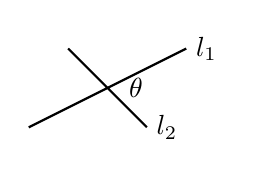
\begin{tikzpicture}[line join=round, scale=0.5]
\coordinate                                   (l11) at (-2,-1);
\coordinate[label=right:{$\boldsymbol{l}_1$}] (l12) at (2,1);
\coordinate                                   (l21) at (-1,1);
\coordinate[label=right:{$\boldsymbol{l}_2$}] (l22) at (1,-1);
\coordinate[label=right:{$\theta $}]          (t)   at (0.3,0);
\draw[thick] (l11)--(l12) (l21)--(l22);
\end{tikzpicture}
\end{minipage}
\begin{minipage}{.32\textwidth}
\centering
\begin{tikzpicture}[style={x={(-135:0.5)},y={(1cm,0)},z={(0,1cm)}}, line join=round, scale=0.3]
\draw (3,-2,0)--(3,6,0)--(-3,6,0)--(-3,-2,0)--(3,-2,0);
\coordinate                                       (A) at (0,0,0);
\coordinate                                       (Q) at (0,4,0);
\coordinate                                       (P) at (0,4,3);
\coordinate[label=above left: {$\boldsymbol{l}$}] (l) at ($(A)!0.5!(P)$);
\coordinate[label=right:      {$\boldsymbol{n}$}] (n) at (P);
\coordinate[label=above right:{$\theta $}]        (t) at (0,1,0);
\draw[thick] (A)--(Q);
\draw[thick,-stealth] (A)--(P);
\draw[thick,-stealth] (Q)--(P);
\end{tikzpicture}
\end{minipage}
\begin{minipage}{.32\textwidth}
\centering
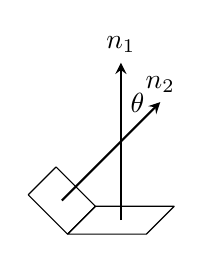
\begin{tikzpicture}[style={x={(-135:0.5)},y={(1cm,0)},z={(0,1cm)}}, line join=round, scale=0.5]
\draw (1,2,0)--(1,0,0)--(-1,0,0)--(-1,2,0)--(1,2,0);
\draw (1,0,0)--(1,-1,1)--(-1,-1,1)--(-1,0,0)--(1,0,0);
\coordinate[label=above:      {$\boldsymbol{n}_1$}] (n1) at (0,1,4);
\coordinate[label=above:      {$\boldsymbol{n}_2$}] (n2) at (0,2,3);
\coordinate[label=above right:{$\theta $}]          (t)  at (0,1,2.5);
\draw[thick,-stealth] (0,1,0)--(n1);
\draw[thick,-stealth] (0,-0.5,0.5)--(n2);
\end{tikzpicture}
\end{minipage}
\end{figure}

\begin{tcolorbox}
本节的例1、例2、例3、例9、例10,都值得反复阅读。
\end{tcolorbox}

%============================================================
\subsection{习题}

\begin{example}[拓广探索18,难度:$\star \star \star $]
在如图所示的实验装置中,两个正方形框架$ABCD$,$ABEF$的边长都是1,且它们所在的平面互相垂直。活动弹子$M,N$分别在正方形对角线$AC$和$BF$上移动,且$CM$和$BN$的长度保持相等,记$CM=BN=a,0<a<\sqrt{2}$。
\begin{enumerate}
    \item 求$MN$的长;
    \item $a$为何值时,$MN$的长最小?
    \item 当$MN$的长最小时,求平面$MNA$和$MNB$夹角的余弦值。
\end{enumerate}
\end{example}

\begin{figure}[h]
\centering
\begin{tikzpicture}[style={x={(-145:0.8)},y={(1cm,-0.2cm)},z={(0,1cm)}}, line join=round, scale=2]
\pgfmathparse{0.6/2}
\mydrawxyz{0}{1.4}{0}{1.4}{0}{1.4}
\coordinate[label=above right:{$B$}] (B) at (0,0,0);
\coordinate[label=below:      {$A$}] (A) at (1,0,0);
\coordinate[label=right:      {$C$}] (C) at (0,0,1);
\coordinate[label=left:       {$D$}] (D) at (1,0,1);
\coordinate[label=above:      {$E$}] (E) at (0,1,0);
\coordinate[label=below:      {$F$}] (F) at (1,1,0);
\coordinate[label=left:       {$M$}] (M) at ($(A)!0.5!(C)$);
\coordinate[label=right:      {$N$}] (N) at ($(B)!0.5!(F)$);
\coordinate[label=left:       {$a$}] (a) at ($(C)!0.5!(M)$);
\coordinate[label=right:      {$a$}] (a) at ($(B)!0.5!(N)$);
\draw[thick] (A)--(B)--(C)--(D)--(A)--(C) (F)--(B)--(E)--(F)--(A) (A)--(N) (B)--(M);
\draw[thick,blue] (M)--(N);
\fill (M) circle (\pgfmathresult mm);
\fill (N) circle (\pgfmathresult mm);
\fill[blue!50!white,opacity=0.5] (M)--(N)--(B)--cycle;
\fill[pink!50!white,opacity=0.5] (M)--(N)--(A)--cycle;
\end{tikzpicture}
\end{figure}

解:

(1)以$B$为原点建立直角坐标系。根据关系可得$M,N$坐标$M=\left( x,0,1-x \right) ,N=\left( x,x,0 \right) $,其中$\sqrt{2}x=a$,于是:
\[
MN=\sqrt{x^2+\left( 1-x \right) ^2}=\sqrt{2x^2-2x+1}=\sqrt{\left( \sqrt{2}x-\frac{1}{\sqrt{2}} \right) ^2+\frac{1}{2}}
\]

(2)可见,当$x=\frac{1}{2}$时,$MN$最小,为$\sqrt{\frac{1}{2}}$,此时$a=\frac{\sqrt{2}}{2}$。

(3)不难发现$\bigtriangleup AMN,\bigtriangleup BMN$均为等边三角形,后略。

深入分析:

探讨一下$MN$最值。首先有一个直觉,高中阶段的不等值最终都可以归结为基本不等式,$MN$两头都是$CB=AF=1$,一定是对称点取到最值,事实也是如此。另一个直觉,异面直线距离最短,$MN$应该是距离,但显然结果的$MN$并不是距离,这点从$MN$和$AC,BF$都不垂直可以得出。两个直觉发生矛盾了。

假设$M,N$各自运动,我们看看什么时候$MN$最短。
另$M,N$坐标$M=\left( x_m,0,1-x_m \right) ,N=\left( x_n,x_n,0 \right) $,于是:
\begin{align*}
MN&=\sqrt{\left( x_m-x_n \right) ^2+{x_n}^2+\left( 1-x_m \right) ^2} \\
&=\sqrt{2{x_m}^2-2x_mx_n+2{x_n}^2+1-2x_m}
\end{align*}
另$y=2{x_m}^2-2x_mx_n+2{x_n}^2+1-2x_m$,计算一阶和二阶偏导:
\begin{align*}
&\because \begin{cases}
	\frac{\partial y}{\partial x_m}=4x_m-2x_n-2=0\\
	\frac{\partial y}{\partial x_n}=-2x_m+4x_n=0\\
\end{cases} \quad \begin{cases}
	A=\frac{\partial ^2y}{{\partial x_m}^2}=4\\
	C=\frac{\partial ^2y}{{\partial x_n}^2}=4\\
	B=\frac{\partial ^2y}{\partial x_m\partial x_n}=-2\\
\end{cases} \\
&\therefore x_m=\frac{2}{3},x_n=\frac{1}{3}
\end{align*}
由于$AC>B,A>0$,所以该值为最小值,此时:
\begin{align*}
&M=\left( \frac{2}{3},0,\frac{1}{3} \right) ,N=\left( \frac{1}{3},\frac{1}{3},0 \right) \\
&MN=\sqrt{\left( 1/3 \right) ^2+\left( 1/3 \right) ^2+\left( 1/3 \right) ^2}=1/\sqrt{3}
\end{align*}
再考察$\bigtriangleup AMN$:
\begin{align*}
&A=\left( 1,0,0 \right) \\
&AM=\sqrt{\left( 1/3 \right) ^2+\left( 1/3 \right) ^2}=\sqrt{2}/\sqrt{3} \\
&AN=\sqrt{\left( 2/3 \right) ^2+\left( 1/3 \right) ^2}=\sqrt{5}/\sqrt{3}
\end{align*}
可见$\bigtriangleup AMN$为直角三角形,同理$\bigtriangleup BMN$也为直角三角形,此刻$MN$垂直于$AC,BF$,$MN$确实是距离。

分析可得,这两个直觉的矛盾在于$M,N$两点的运动方式,若无约束确实可以取到距离,但题目对它们的运动方式有了约束,所以取不到距离。

\begin{tcolorbox}
本题采用向量的方法将几何问题转化为代数问题,需要将几何和代数融会贯通,但总体上思路还是明确的。
\end{tcolorbox}




